
\documentclass{beamer}
\mode<presentation>{ \usetheme{boxes} }

\usepackage[utf8]{inputenc}
\usepackage[spanish]{babel}
\usepackage{amsmath, amsthm, amsfonts}
\usepackage{verbatim}
\usepackage{graphicx}
\usepackage{subfigure}

\title {DESARROLLO DE UN SISTEMA PROTOTIPO DE RECONOCIMIENTO DE DÍGITOS USANDO MOMENTOS INVARIANTES}
\author { Sebastián Gómez González \\ Santiago Gutierrez Alzate}
\date {Junio de 2011}

\usetheme{Warsaw}
\begin{document}

	\frame{\titlepage}
	
	\frame{\tableofcontents}
	
	\section{Introducción}
	\subsection{Formulación del problema}
	\begin{frame}
		\frametitle{Formulación del problema}
		\begin{itemize}
			\item Según el DANE en su gran censo nacional realizado en el año 2005, se estima que el 6.3\% de la población colombiana sufre de alguna discapacidad. De estas personas con discapacidad se estima que el 43.4\% tienen dificultades para ver aun con lentes.\pause
			\item La organización mundial de la salud estima que en el mundo hay 161 millones de personas con problemas visuales, de los cuales 37 millones son ciegos.\pause
			\item No se encontró un sistema de reconocimiento de caracteres por un medio óptico que haya sido desarrollado para ser usado por personas invidentes en teléfonos inteligentes, que sea de código libre y abierto 
		\end{itemize}
	\end{frame}
	
	\subsection{Justificación}
	\begin{frame}
		\frametitle{Justificación}
		\begin{itemize}
			\item Un menor costo, al no ser necesario adquirir un computador de escritorio, escáner o impresora braille. \pause
			\item Portabilidad.\pause
			\item Una solución económica que pueda ejecutarse en un dispositivo móvil.\pause
			\item Aportar al conocimiento.
		\end{itemize}
	\end{frame}
	
	\begin{frame}
		\frametitle{Objetivo del proyecto}
		\begin{block}{Objetivo General}
		Desarrollar un sistema prototipo de reconocimiento óptico de dígitos numéricos bajo condiciones especificadas, usando para el reconocimiento una distribución normal multivariable con el teorema de Bayes y un vector de características invariantes (momentos de Hu y Flusser).
		\end{block}
		\pause
		\begin{block}{Objetivos específicos}
			\begin{itemize}
			\item Realizar un estudio del funcionamiento de la distribución normal multivariable para dar solución a problemas de reconocimiento en general utilizando el teorema de Bayes. 
			\item Realizar la extracción de características de un conjunto de imágenes de dígitos. Las características a extraer serán invariantes a la rotación, translación y escalamiento (Momentos de Hu y Flusser).
			\item Diseñar e implementar una aplicación que integre estos algoritmos y permita el reconocimiento óptico de dígitos.
			\item Realizar pruebas de la aplicación implementada.
			\item Realizar un análisis comparativo de los resultados obtenidos. 
			\end{itemize}
		\end{block}
	\end{frame}
	
	\subsection{Etapas}
	\begin{frame}
		\frametitle{Etapas de un sistema OCR}
		\begin{block}{Etapas del sistema completo}
		\begin{itemize}
			\item Análisis del documento \pause
			\item Reconocimiento óptico de caracteres (OCR) \pause
			\item Conversión de texto a voz (TTS)\pause
		\end{itemize}
		\end{block}
		\begin{block}{Etapas del OCR}
		\begin{itemize}
			\item Etapas de preprocesamiento. \pause
			\item Extracción de características. \pause
			\item Reconocimiento usando aprendizaje de máquinas.
		\end{itemize}
		\end{block}
	\end{frame}
	
	
	\section{Extracción de características de los caracteres}
	
	\subsection{Preprocesamiento}
	
	\begin{frame}
		\frametitle{Conversión a escala de grises}
		\begin{equation}\label{eq:bwtocv}
			gris = 0.2989 * rojo + 0.5870 * verde + 0.1140 * azul 
		\end{equation}
	\end{frame}
	
	\begin{frame}
	\frametitle{Binarización}
	Un método muy utilizado para binarizar una imagen es escoger un valor umbral $T(x,y)$ para cada píxel $(x,y)$ y establecer el valor de cada píxel como:
	\begin{equation}\label{binEq}
	I_2(x,y) = \left\{ \begin{array}{ll}
		0   & \mbox{si $I_1(x,y) < T(x,y)$} \\
		255 & \mbox{en cualquier otro caso}
	\end{array} \right. 
	\end{equation}
	
	Donde $I_1(x,y)$ es la imagen original y $I_2(x,y)$ es la imagen binarizada. 
	\end{frame}
	
	\begin{frame}
	\frametitle{Método de Sauvola}
	El valor umbral se calcula con el método de Sauvola:
	
	\begin{equation}\label{rSauvola}
	T(x,y)=m(x,y)\left[ 1 + k(\frac{s(x,y)}{R}-1) \right]
	\end{equation}
	
	Donde $m(x,y)$ es la media y $s(x,y)$ la desviación estándar de los píxeles en algún área alrededor de $(x,y)$, y R es el máximo valor de la desviación estándar (128 para una imagen en escala de grises). 
	
	La complejidad computacional de calcular $T(x,y)$ para todos los píxeles de una imagen de tamaño $N \times M$ sería $O(N \times M \times A^{2})$.
	\end{frame}
	
	\begin{frame}
	\frametitle{Optimización de Breuel}
	\begin{align*}
	  m(x, y) =& (I(x + \frac{A}{2}, y + \frac{A}{2}) + I(x - \frac{A}{2}, y - \frac{A}{2}) \\
		   &- I(x + \frac{A}{2}, y - \frac{A}{2}) - I(x - \frac{A}{2}, y + \frac{A}{2})) / A^{2}
	\end{align*}

	\begin{figure}[htb]
	\begin{center}
	\leavevmode
	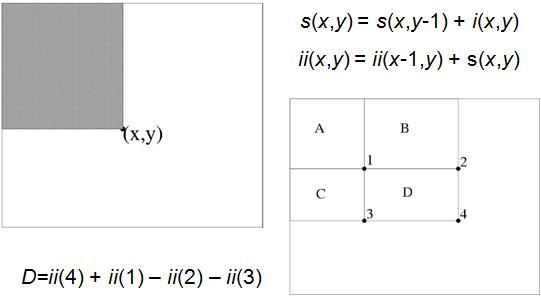
\includegraphics[width=6cm]{img/integral.png}
	\end{center}
	\caption{Imagen integral (Tomado de ACM Student Reseach Competition)}
	\label{fig:integral}
	\end{figure}
	\end{frame}
	
	\begin{frame}
	\frametitle{Ejemplo de imagen Binarizada}
	\begin{figure}
	\centering
		\subfigure[Antes de binarizar]{\label{fig:bin1}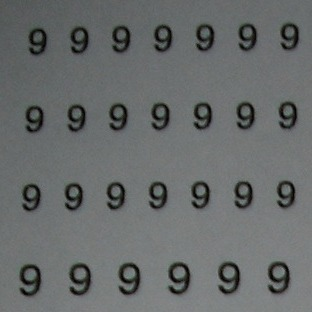
\includegraphics[width=4cm]{img/bin1.jpg}}
		\subfigure[Después de binarizar]{\label{fig:bin2}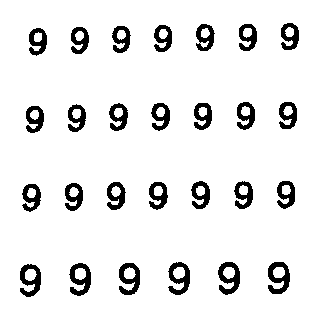
\includegraphics[width=4cm]{img/bin2.png}}
	\caption{Figuras antes y después de la binarización}
	\label{fig:binarization}
	\end{figure}
	\end{frame}
	
	\subsection{Componentes conectados}
	\begin{frame}
	\frametitle{Componentes conectados}
	\begin{figure}
	\centering
		\subfigure{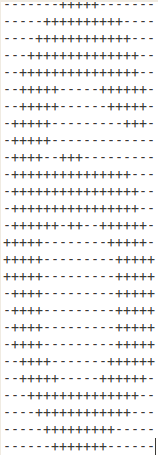
\includegraphics[width=2cm]{img/p1.png}}
		\hspace{1cm}
		\subfigure{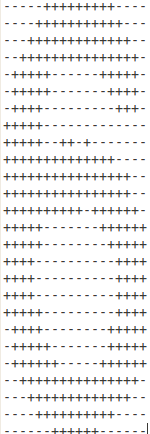
\includegraphics[width=2cm]{img/p2.png}}\\		
	\caption{Componentes conectados extraídos por la aplicación}
	\label{fig:concomp}
	\end{figure}
	\end{frame}
	
	\subsection{Extracción de características}
	\begin{frame}
	\begin{block}{Las características deben ...}
	\begin{itemize}
		\item Permitir diferenciar los distintos símbolos independiente de el tamaño o la inclinación.
		\item Ser vectores de números reales que aporten la mayor cantidad de información con un mínimo de dimensiones.
	\end{itemize}
	\end{block}
	\end{frame}
	
	\begin{frame}
		\frametitle{Distintos enfoques}
		\begin{block}{Corrección de la inclinación}
		\begin{itemize}
			\item Se debe hallar el ángulo de rotación
			\item Se pierde información cuando el ángulo no es múltiplo de $90^\circ$
		\end{itemize}
		\[
		\begin{pmatrix} 
			x' \\ y'
		\end{pmatrix}
		=
		\begin{pmatrix} 
			\cos\theta & -\sin\theta \\
			\sin\theta & \cos\theta
		\end{pmatrix}
		\begin{pmatrix} 
			x \\ y
		\end{pmatrix}
		\]
		\end{block}
		
		\begin{block}{Momentos Invariantes}
		\begin{itemize}
			\item Entrega vectores numéricos que son idealmente independiente de la rotación
			\item No se requiere hacer corrección del ángulo de inclinación de la imagen
			\item Existen diferentes enfoques, se utilizaran los momentos de Hu, Flusser y Flusser para simetría N-Fold.
		\end{itemize}
		\end{block}
	\end{frame}
	
	\begin{frame}
	\frametitle{Momentos invariantes de Hu}
	Momentos geométricos invariantes a la translación:
	\begin{equation}\label{eq1}
		\mu_{pq} = \iint{ {(x-\bar{x})^p} {(y-\bar{y})^q} f(x,y) dy dx }
	\end{equation}
	Invariantes al escalamiento:
	\begin{equation}\label{eq2}
		n_{pq} = \frac{\mu_{pq}}{ \mu_{00}^{1+\frac{p+q}{2}} }
	\end{equation}
	
	\end{frame}

	\begin{frame}
	\frametitle{Momentos invariantes de Hu}
	\begin{align}
		\phi_1 =& n_{20} + n_{02}, \notag\\ 
		\phi_2 =& (n_{20} - n_{02})^{2} + 4n_{11}^{2}, \notag \\ 
		\phi_3 =& (n_{30} - 3n_{12})^{2} + (3n_{21} - n_{03})^{2}, \notag \\ 
		\phi_4 =& (n_{30} + n_{12})^{2} + (n_{21} + n_{03})^{2},\notag \\ 
		\phi_5 =& (n_{30} - 3n_{12})(n_{30} + n_{12})((n_{30} + n_{12})^{2} \notag \\
				& - 3(n_{21} + n_{03})^{2}) + (3n_{21} - n_{03})(n_{21} + n_{03})\notag\\ 
				& \times (3(n_{30} + n_{12})^{2} - (n_{21} + n_{03})^{2}),\notag\\ 
		\phi_6 =& (n_{20} - n_{02})((n_{30} + n_{12})^{2} - (n_{21} + n_{03})^{2})\notag\\
				& + 4n_{11}(n_{30} + n_{12})(n_{21} + n_{03}),\notag\\
		\phi_7 =& (3n_{21} - n_{03})(n_{30} + n_{12})((n_{30} + n_{12})^{2}\notag\\
				& - 3(n_{21} + n_{03})^{2}) - (n_{30} - 3n_{12})(n_{21} + n_{03}) \notag\\
				& \times (3(n_{30} + n_{12})^{2} - (n_{21} + n_{03})^{2}) \label{eq:huMom} \\ \notag
	\end{align}
	\end{frame}
	
	\subsection{Momentos de Flusser}
	\begin{frame}
	\frametitle{Momentos invariantes de Flusser}
	En 1984 Mostafa y Psaltis propusieron los momentos complejos como una forma alternativa de lograr momentos invariantes. Un momento complejo $C_{pq}$ de orden $(p+q)$ para una imagen $f(x,y)$ se define como:

	\[ C_{pq} = \iint{ (x+iy)^p (x-iy)^q f(x,y) dx dy } \]
	
Donde i denota la unidad imaginaria. En coordenadas polares esto es equivalente a:

	\begin{equation}\label{eq:polarCplx}
		C_{pq} = \iint{ r^{p+q+1}e^{i(p-q)\theta}f(r,\theta) dr d\theta }
	\end{equation}
	\end{frame}
	
	\begin{frame}
	\frametitle{Momentos invariantes de Flusser}
	Sea $f'(r,\theta) = f(r,\theta+\alpha)$ entonces:

	\begin{equation}\label{eq:rotProp}
		C'_{pq} = e^{-i(p-q)\alpha}C_{pq}
	\end{equation}

	Donde $C'_{pq}$ es el momento complejo de $f'(r,\theta)$ y $C_{pq}$ es el momento complejo de $f(r,\theta)$
	\end{frame}
	
	
	\section{Métodos estadísticos de clasificación}
	
	\subsection{Introducción}
	\begin{frame}
	\frametitle{Modelo general de un clasificador}
	\begin{figure}[htb]
	\begin{center}
	\leavevmode
	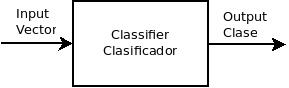
\includegraphics[width=5cm]{diagrams/classifier1.jpg}
	\end{center}
	\caption{Modelo general de un clasificador}
	\label{fig:classif1}
	\end{figure}
	\end{frame}
	
	\subsection{Algunos algoritmos de clasificación}
	
	\begin{frame}
	\frametitle{Árboles binarios de decisión}
	\begin{figure}[htb]
	\begin{center}
	\leavevmode
	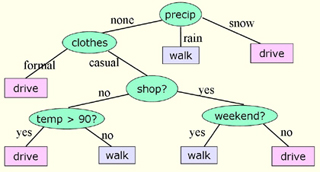
\includegraphics[width=7cm]{img/decisiontree.jpg}
	\end{center}
	\caption{Ejemplo de árbol de decisión, tomado de MIT OpenCourseware.}
	\label{fig:decisionTree}
	\end{figure}
	\end{frame}
	
	\begin{frame}
	\frametitle{Árboles binarios de decisión}
	\begin{block}{Características}
	\begin{itemize}	
	\item Son fácilmente interpretables por un ser humano. \pause
	\item En general son más efectivos en los problemas que tienen entradas discretas. \pause	
	\item Si el árbol esta balanceado correctamente la velocidad de clasificación es alta. \pause	
	\item Se debe optimizar la profundidad máxima del árbol, pues un valor adecuado es importante para obtener un buen resultado. \pause
	\item El poder clasificatorio de los árboles es limitado, especialmente si se comparan con otros algoritmos de clasificación. \pause	
	\item La mayoría de algoritmos existentes para generar árboles de decisión solo permiten condiciones sobre una única variable por nodo. En estos casos se limita aun más su poder clasificatorio. 
	\end{itemize}
	\end{block}
	\end{frame}
	
	\begin{frame}
	\frametitle{Métodos estadísticos}
	\begin{block}{Características}
	\begin{itemize}
	\item No necesita configuración, lo único que se debe saber en un método estadístico a-priori es la distribución de probabilidad con la que se va a aproximar el modelo real. \pause
	\item Un modelo estadístico es fácil de interpretar por un humano, aunque no es tan fácil de interpretar como los árboles de decisión. \pause
	\item El poder clasificatorio es más alto que el de los árboles de decisión. \pause
	\item Brinda mucha información, en vez de solo determinar a qué clase pertenece una instancia, brida la probabilidad de que la instancia pertenezca cada una de las demás clases.
	\end{itemize}
	\end{block}
	\end{frame}
	
	\begin{frame}
	\frametitle{Redes Neuronales Artificiales}
	\begin{figure}[htb]
	\begin{center}
	\leavevmode
	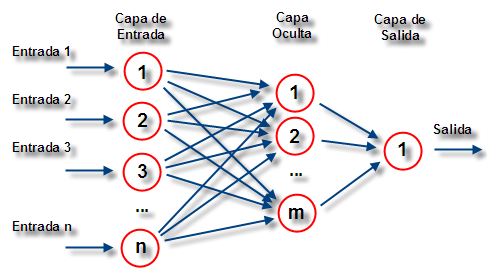
\includegraphics[width=7cm]{img/rna.png}
	\end{center}
	\caption{Ejemplo de un perceptrón con una capa oculta, tomado de Wikimedia}
	\label{fig:rna}
	\end{figure}
	\end{frame}
	
	\begin{frame}
	\frametitle{Redes Neuronales Artificiales}
	\begin{block}{Características}
	\begin{itemize}
	\item El poder clasificatorio de este método es mayor que el de los métodos anteriormente mencionados. Matemáticamente se ha demostrado que no exigen ninguna distribución determinada de los datos, ni tampoco que estos sean separables linealmente. \pause
	\item Al igual que el método estadístico, con una función de activación adecuada se puede calcular la probabilidad de que una instancia pertenezca a cada clase. \pause
	\item Dada la cantidad de parámetros que se pueden configurar, estos algoritmos son muy difíciles de afinar para un problema determinado. \pause
	\item Las redes neuronales son difíciles de interpretar. Una vez entrenadas pueden dar buenos o malos resultados, pero es difícil saber cuál es el error real, o si es posible mejorar los resultados cambiando los parámetros. 
	\end{itemize}
	\end{block}
	\end{frame}
	
	\subsection{Distribución Normal Multivariable}
	
	\begin{frame}
	\frametitle{La distribución normal}
	\begin{equation}
		p(x) = \frac{1}{\sqrt{2\pi}\sigma}exp\left[-\frac{(x-\mu)^2}{2\sigma^2}\right]
	\label{eq:normal}
	\end{equation}
	Donde $exp[x]$ es la función exponencial $e^x$, $\mu$ son la media y $\sigma$ se conoce como desviación estándar
	\end{frame}
	
	\begin{frame}
	\frametitle{Distribución Normal Multivariable}
	Supongamos que tenemos un vector d-dimensional $\vec{x}$ que sigue una distribución normal multivariable, entonces:

	\begin{equation}\label{eq:multDens}
		p(x) = \frac{1}{(2\pi)^{d/2}|\Sigma|^\frac{1}{2}} exp\left[{-\frac{1}{2}(\vec{x}-\vec{\mu})\Sigma^{-1}(\vec{x}-\vec{\mu})}\right]
	\end{equation}

Esto se denota como $\vec{x} \sim N(\vec{\mu},\Sigma)$ y significa que $\vec{x}$ sigue una distribución normal multivariable cuya media es el vector $\vec{\mu}$ y cuya matriz de covarianza es la matriz $\Sigma$
	\end{frame}
	
	\begin{frame}
	\frametitle{Distribución Normal Multivariable}
	Si para cada clase $C_i$ se calculan la media $\vec{\mu_i}$ y la matriz de covarianza $\Sigma_i$, la densidad de probabilidad $p(x|C_i)$ es:

	\begin{equation}\label{eq:multivariate}
		p(x|C_i) = \frac{1}{(2\pi)^{d/2}|\Sigma_i|^\frac{1}{2}} exp\left[{-\frac{1}{2}(\vec{x}-\vec{\mu_i})\Sigma_i^{-1}(\vec{x}-\vec{\mu_i})}\right]
	\end{equation}
	
	Usando el teorema de Bayes se tiene:
	
	\begin{equation}\label{eq:multBayes}
		P(C_i|\vec{x}) = \frac{p(\vec{x}|C_i)P(C_i)}{p(x)} = \frac{p(\vec{x}|C_i)P(C_i)}{ \sum_j{p(\vec{x}|C_j)P(C_j)} }
	\end{equation}
	\end{frame}
	
	\begin{frame}
	\frametitle{Entrenamiento}
	\begin{equation}\label{eq:multiParams}
	\begin{aligned}
		\vec{\mu_i} &= E[ \vec{x_i} ] \\
		\Sigma_i(a,b) &= E[ (\vec{x_i}-\vec{\mu_a})(\vec{x_i}-\vec{\mu_b}) ]
	\end{aligned}
	\end{equation}

	Donde $\vec{x_i}$ son las instancias del conjunto $T_i$, $E[x]$ es el valor esperado o media de $x$ y $\Sigma_i(a,b)$ es el valor en la fila $a$ y la columna $b$ de la matriz $\Sigma_i$.
	\end{frame}
	
	\begin{frame}
	\frametitle{Matriz de covarianza semi-compartida}
	Se plantea un método en el que se comparte la matriz de covarianza en el coeficiente pero no en el exponente.
	\begin{equation}\label{eq:semishared}
		p(x|C_i) = \frac{1}{(2\pi)^{d/2}|\Sigma|^\frac{1}{2}} e^{-\frac{1}{2}(\vec{x}-\vec{\mu_i})\Sigma_i^{-1}(\vec{x}-\vec{\mu_i})}
	\end{equation} 
	\end{frame}
	
	\section{Resultados}
	
	\subsection{Primeros resultados}
	\begin{frame}
	\frametitle{Primeros resultados}
	\begin{table}
	\centering
	\begin{tabular}{|c|p{3cm}|p{3cm}|}
		\hline
		* & \multicolumn{2}{|c|}{Matriz de covarianza independiente} \\
		\hline
		Caracter & Hu & Flusser \\
		\hline
		0 & 99.86\% & 100.00\% \\
		1 & 100.00\% & 100.00\% \\
		2 & 91.21\% & 93.91\% \\
		3 & 100.00\% & 100.00\% \\
		4 & 100.00\% & 96.41\% \\		
		5 & 26.95\% & 38.95\% \\ 
		6 & 93.61\% & 86.83\% \\
		7 & 100.00\% & 99.87\% \\
		8 & 96.76\% & 99.44\% \\
		9 & 65.40\% & 65.03\% \\
		\hline
		Total & 87.21\% & 87.84\% \\
		\hline
	\end{tabular}
	\caption{Precisión del algoritmo clasificador en el primer experimento}	
	\label{tb:exp1_1}
	\end{table}
	\end{frame}
	
	\begin{frame}
	\frametitle{Primeros resultados}
	\begin{table}
	\begin{center}
	\begin{tabular}{|c|p{3cm}|p{3cm}|}
		\hline
		* & \multicolumn{2}{|c|}{Matriz de covarianza semi-compartida} \\
		\hline
		Caracter & Hu & Flusser \\
		\hline
		0 & 99.34\% & 99.21\% \\
		1 & 100.00\% & 100.00\% \\
		2 & 100.00\% & 100.00\% \\
		3 & 100.00\% & 100.00\% \\
		4 & 100.00\% & 100.00\% \\		
		5 & 97.97\% & 99.32\% \\ 
		6 & 91.65\% & 86.96\% \\
		7 & 100.00\% & 100.00\% \\
		8 & 85.53\% & 92.97\% \\
		9 & 89.52\% & 81.06\% \\
		\hline
		Total & 96.38\% & 95.83\% \\
		\hline
	\end{tabular}
	\end{center}
	\caption{Precisión del algoritmo clasificador en el segundo experimento}	
	\label{tb:exp1_2}
	\end{table}
	\end{frame}
	
	\subsection{Problemas de simetría mutua}
	
	\begin{frame}
	\frametitle{Problemas de simetría mutua}
	Recordemos la ecuación \ref{eq:rotProp}:
	\[ C'_{pq} = e^{-i(p-q)\alpha}C_{pq} \]
	Donde $C'_{pq}$ es el momento complejo de referencia y $C_{pq}$ el momento complejo de la imagen $f(x,y)$.
	\begin{equation}\label{eq:angleDetection1}
		\frac{C'_{pq}}{C_{pq}} = e^{-i(p-q)\alpha}
	\end{equation}
	Definamos $n=\frac{C'_{pq}}{C_{pq}}$, con $p \neq q$. Y definamos $n'=\frac{n}{|n|}$.
	\begin{equation}\label{angleDetection2}
		n' = \cos((p-q)\alpha) - i\sin((p-q)\alpha)
	\end{equation}	
	\end{frame}
	
	\begin{frame}
	\frametitle{Problemas de simetría mutua}
	\begin{center}
	\setlength{\unitlength}{1cm}
	\begin{figure}
	\centering
	\begin{picture}(2,2)	
	\put(1,1){\circle{2}}
	\put(1,1){\vector(1,0){0.9}}
	\put(2,1){$\vec{R}$}
	\put(1,0.1){\line(0,1){1.8}}
	\put(1,0){A}
	\put(1,1){\vector(1,2){0.4}}
	\put(1.5,1.8){$n'$}
	\end{picture}	
	\caption{Clasificación de figuras con simetría mutua dado el plano $A$}
	\label{fig:mutualSym}
	\end{figure}
	\end{center}
	
	\[ \vec{R}.n' = real(n') \]
	
	Donde $real(x)$ es una función que retorna la parte real del número complejo $x$. La clasificación se realizo de la siguiente forma:

	\begin{equation}\label{angleClassif}
		Class = \left\{ \begin{array}{ll}
		C_i   & \mbox{if $real(n') > 0$} \\
		C_j & \mbox{otherwise}
	\end{array} \right. 
	\end{equation}
	\end{frame}
	
	\begin{frame}
	\frametitle{Resultados luego de la corrección del 6 y el 9}
	\begin{table}
	\begin{center}
	\begin{tabular}{|c|p{3cm}|p{3cm}|}
		\hline
		* & \multicolumn{2}{|c|}{Matriz de covarianza semi-compartida} \\
		\hline
		Caracter & Hu & Flusser \\
		\hline
		0 & 99.34\% & 99.21\% \\
		1 & 100.00\% & 100.00\% \\
		2 & 100.00\% & 100.00\% \\
		3 & 100.00\% & 100.00\% \\
		4 & 100.00\% & 100.00\% \\		
		5 & 97.97\% & 99.32\% \\ 
		6 & 99.47\% & 99.48\% \\
		7 & 100.00\% & 100.00\% \\
		8 & 85.53\% & 92.97\% \\
		9 & 99.49\% & 96.72\% \\
		\hline
		Total & 98.18\% & 98.77\% \\
		\hline
	\end{tabular}
	\end{center}
	\caption{Precisión al aplicar la mejora (6 y 9)}	
	\label{tb:exp2_2}
	\end{table}
	\end{frame}
	
	\subsection{Problemas de simetría a la rotación}
	
	\begin{frame}
	\frametitle{Momentos de Flusser para la simetría a la rotación}
	Flusser demostró que muchos de estos momentos son iguales a cero cuando los objetos que se intentan reconocer con ellos tienen algún grado de simetría y, para solucionar este problema, propuso un nuevo método para generar momentos adecuados para reconocer objetos con simetría de grado N.
	\newline \newline
	Las pruebas siguientes se realizaron sobre un conjunto de validación de 7461 instancias.
	\end{frame}
	
	\begin{frame}
	\frametitle{Momentos de Flusser para la simetría a la rotación}
	\begin{table}
	\begin{center}
	\begin{tabular}{|c|c|c|c|}
		\hline
		* & \multicolumn{3}{|c|}{Matriz de covarianza independiente} \\
		\hline
		Caracter & Hu & Flusser & 2-Fold Flusser\\
		\hline
		0 & 99.86\% & 100.00\% & 100.00\%\\
		1 &	100.00\% & 100.00\% & 100.00\% \\
		2 &	91.21\% & 93.91\% & 47.14\% \\
		3 &	100.00\% & 100.00\% & 99.42\% \\
		4 &	100.00\% & 96.41\% & 100.00\% \\		
		5 & 26.95\% & 38.95\% & 100.00\% \\ 
		6 & 93.61\% & 99.48\% & 100.00\% \\
		7 & 100.00\% & 99.87\% & 100.00\% \\
		8 & 96.76\% & 99.44\% & 100.00\% \\
		9 &	65.40\% & 96.72\% & 100.00\% \\
		\hline
		Total & 87.38\% & 92.47\% & 94.44\% \\
		\hline
	\end{tabular}
	\end{center}
	\caption{Precisión del clasificador en los tres experimentos}	
	\label{tb:exp4_1}
	\end{table}
	\end{frame}
	
	\begin{table}
	\begin{center}
	\begin{tabular}{|c|p{2cm}|p{2cm}|p{2cm}|}
		\hline
		* & \multicolumn{3}{|c|}{Matriz de covarianza semi-compartida} \\
		\hline
		Caracter & Hu & Flusser & 2-Fold Flusser\\
		\hline
		0 & 99.34\% & 99.21\% & 100.00\% \\
		1 & 100.00\% & 100.00\% & 100.00\% \\
		2 & 100.00\% & 100.00\% & 100.00\% \\
		3 & 100.00\% & 100.00\% & 100.00\% \\
		4 & 100.00\% & 100.00\%	& 100.00\% \\		
		5 & 97.97\% & 99.32\% & 100.00\% \\ 
		6 & 99.47\% & 99.48\% & 100.00\% \\
		7 & 100.00\% & 100.00\% & 100.00\% \\
		8 & 85.53\% & 92.97\% & 100.00\% \\
		9 & 99.49\% & 96.72\% & 100.00\% \\
		\hline
		Total & 98.18\% & 98.77\% & 100.00\% \\
		\hline
	\end{tabular}
	\end{center}
	\caption{Precisión del clasificador en los tres experimentos}	
	\label{tb:exp4_2}
	\end{table}
	
	\subsection{Conclusiones}
	\begin{frame}
	\frametitle{Resultados finales}
	
	\begin{block}{Resultados sobre los dígitos}
	\begin{itemize}
	\item El mejor conjunto de características en todos los casos son los de Flusser para objetos con grado de simetría. \pause
	\item El mejor algoritmo de clasificación en todos los casos es la distribución normal con matriz de covarianza semi-compartida. \pause
	\item La solución planteada para el problema de simetría mutua resolvió efectivamente el problema. \pause
	\end{itemize}
	\end{block}
	
	\begin{block}{Resultados finales sobre el alfabeto}
	\begin{itemize}
	\item Se tomó la decisión de utilizar los algoritmos anteriores para los dígitos (Sobrepasando los objetivos) \pause
	\item Las conclusiones anteriores se mantienen para el alfabeto \pause
	\item El mejor método tiene una efectividad de 99.28\%.
	\end{itemize}
	\end{block}
	
	\end{frame}
	
	\begin{frame}
	\frametitle{Proyectos futuros}
	\begin{itemize}
	\item Optimizar el sistema de reconocimiento de caracteres para el reconocimiento de letras mayúsculas y minúsculas. \pause
	\item Soportar distintos tipos de letra (fuentes) en el sistema OCR. \pause
	\item Desarrollar la etapa de análisis del documento. \pause
	\item Extender el sistema para reconocer otro tipo de objetos.
	\end{itemize}
	\end{frame}
	
\end{document}
